\documentclass[11pt]{article}
\usepackage{lineno}
\usepackage{graphicx}
\usepackage{bm}
\usepackage{graphicx}


\begin{document}





\DeclareGraphicsExtensions{.png,.jpg}



\begin{titlepage}

\newcommand{\HRule}{\rule{\linewidth}{0.5mm}} 

\center % Center everything on the page
 
%----------------------------------------------------------------------------------------
%	HEADING SECTIONS
%----------------------------------------------------------------------------------------

\textsc{\LARGE Texas A$\&$M University}\\[1.5cm] 
\textsc{\Large Preliminary Investigation}\\[0.5cm] % 

%----------------------------------------------------------------------------------------
%	TITLE SECTION
%----------------------------------------------------------------------------------------

\HRule \\[0.4cm]
{ \huge \bfseries Applications of the Abundancy Function in Primality Testing }\\[0.4cm]  %how do you make subtitles this is way too long
\HRule \\[1.5cm]
 
%----------------------------------------------------------------------------------------
%	AUTHOR SECTION
%----------------------------------------------------------------------------------------

\begin{minipage}{0.4\textwidth}
\begin{flushleft} \large
\emph{Authors:}\\
Daniel \textsc{Whatley}\\
Sarah \textsc{Sahibzada}\\
Taylor \textsc{Wilson}
\end{flushleft}
\end{minipage}
~
\begin{minipage}{0.4\textwidth}
\begin{flushright} \large
\emph{Supervisor:} \\
Dr. Sara \textsc{Pollock} 
\end{flushright}
\end{minipage}\\[4cm]

%----------------------------------------------------------------------------------------
%	DATE SECTION
%----------------------------------------------------------------------------------------

{\large \today}\\[3cm] 

%----------------------------------------------------------------------------------------
%	LOGO SECTION
%----------------------------------------------------------------------------------------

%\includegraphics[scale=.3]{tamulogo.png}\\[1cm] 
 
%----------------------------------------------------------------------------------------

\vfill 

\end{titlepage}

\tableofcontents
\newpage
\newpage

\section{Introduction}
\begin{dfn}
Two positive integers $a$ and $b$ are \textit{friendly} if $\sigma(a)/a = \sigma(b)/b$, where $\sigma(n)$ is the sum of the positive integer divisors of $n$.
\end{dfn}

The function $\sigma(n)/n$ is called the \textit{abundancy function}. A positive integer $n$ is called \textit{abundant} if $\sigma(n) > n$, \textit{deficient} if $\sigma(n) < n$, and \textit{perfect} if $\sigma(n) = n$. Thus, all the perfect numbers are pairwise friendly as the abundancy function of each is 1. A number is called \textit{solitary} if it is not friendly with any other number---hence, all prime numbers are solitary.

This investigation also seeks to evaluate the extent to which the abundancy function may be modeled in order to predict prime numbers. In particular, with the consideration that the abundancy of any prime p is $\frac{p+1}{p}$, it is clear that this function will asymptotically approach 1 for prime inputs. This investigation will perform computations to attempt to fit the abundancy curve and verify it against the first million prime numbers. This computation may provide insight into the distribution of primes, and potentially have applications in primality testing.

There are several papers in which some numbers were proven to be solitary, such as 18. There are also papers in which possibilities for friends of 10 are narrowed down.
$ $ \indent 

\section{Theoretical Analysis: Neural Networks}
\subsection{Artificial Neural Networks and their Architectures}

\subsection{The Neuron}


\subsection{Network Architectures}

\subsubsection{Feed-Forward Networks}

\subsubsection{Recurrent Networks}

\subsection{Learning}
 




\section{Computational Approaches}$ $
\subsection{Implementation Detail and Process}
All calculations were performed in Python 2.7, utilizing Matplotlib for graph renderings, excepting curve-fitting, which was performed in Microsoft Excel due to the limited scope of this investigation. Computations were performed on a Linux-based server hosted by Texas A\& M University. 

 Random samples of the first 1000, 10,000, and 100,000 primes were taken to generate curves, with $r^{2}$ values recorded for each. A logarithmic curve was used to fit each data set.

\section{Results}$ $
The abundancy function, when given prime inputs, has results as below:
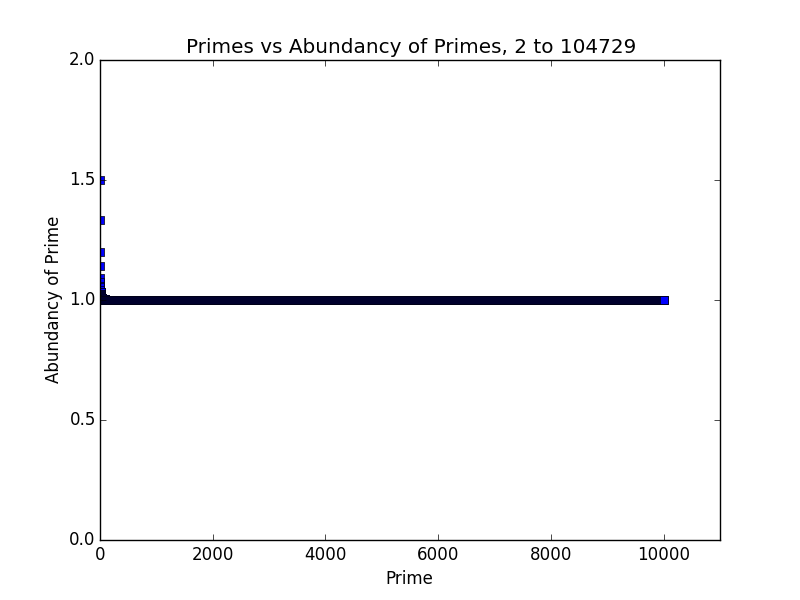
\includegraphics[scale=0.5]{figure_1.png}. 
\\ For all integer inputs, it is as below \\
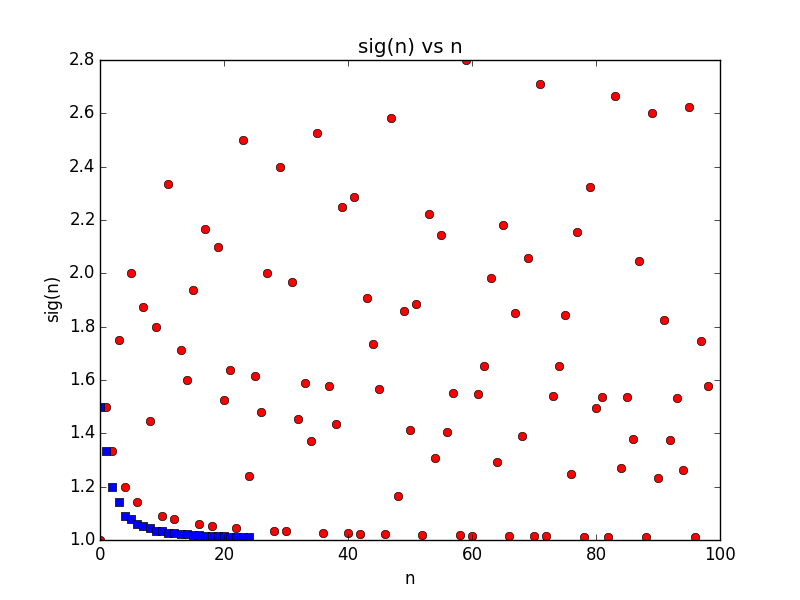
\includegraphics[scale=0.5]{with_primes_small.png}
\\ The ratio of $sig(n)$ to $n$ was also graphed. It is relevant to note that due to the nature of the $sig(n)$ function for prime numbers, there is a strong linear correlation between $sig(n)$ and $n$.
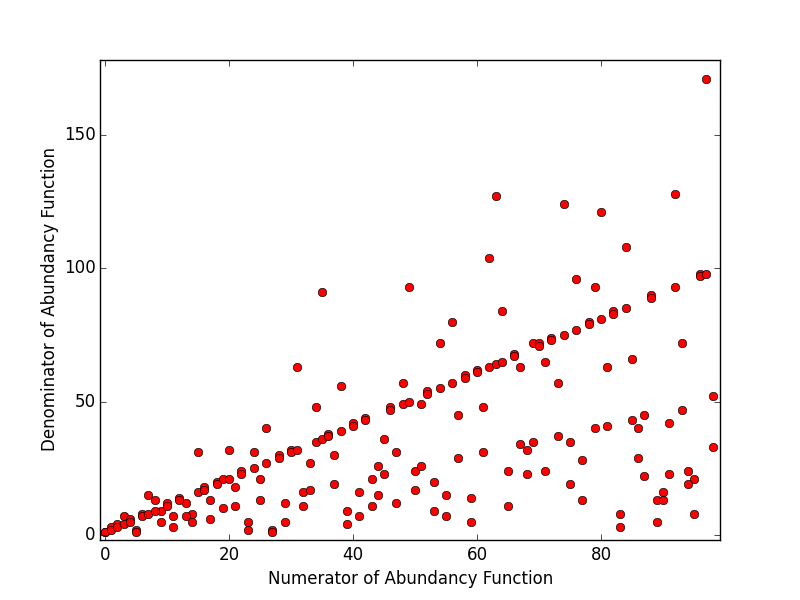
\includegraphics[scale=0.5]{num_vs_denom_1_to_100.png}.



A random sample was taken from the aforementioned subssets of the first million primes using a random number generator from the Random library in Python. Logarithmic regression equations were performed, with the results as below:\\
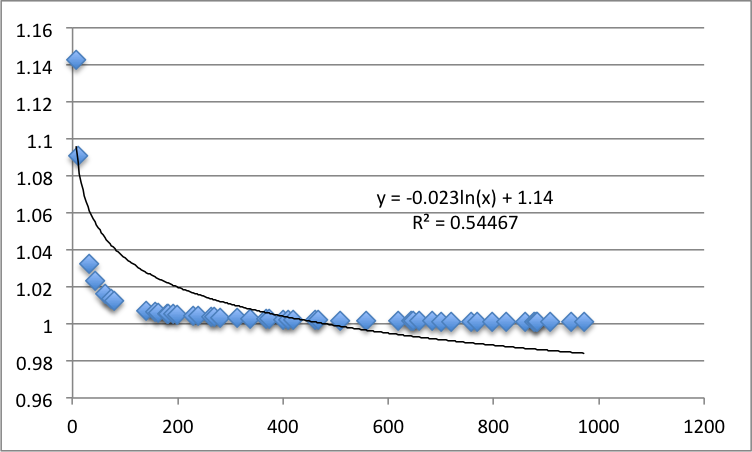
\includegraphics[scale=0.5]{Untitled1.png}
\\ \\
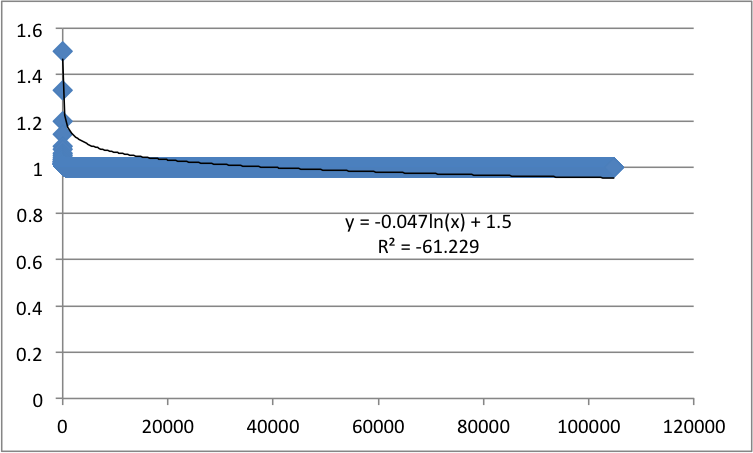
\includegraphics[scale=0.5]{Untitled2.png}
\\
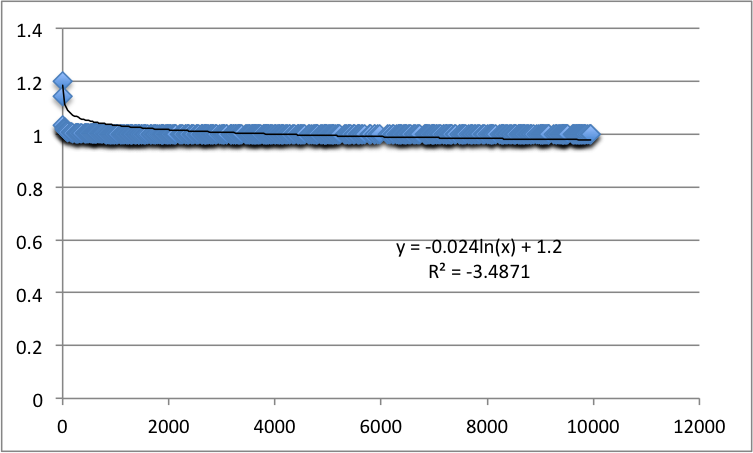
\includegraphics[scale=0.5]{Untitled3.png}

\\ The equations obtained were $-0.047ln(x) + 1.5$, $-0.024ln(x) + 1.2$, and $-0.023ln(x) + 1.14$, where x represents the index of the prime in the set of all primes; respectively, each had $R^{2}$ values of -61.229, -3.4871, and 0.5. Correlations are weak to moderate; two out of the three are negative. When tested, each equation produced zero correct results for primes, implying that while each might be approximately accurate, this curve is in no way capable of replacing a deterministic primality test.
\section{Discussion}$ $

It is clear that the abundancy function cannot be fitted with a logarithmic curve of the form $f(x) = aln(x) + b$. No numbers were correctly matched by any of the equations determined for each sample, and the correlations determined were weak to moderate. It is not possible that the accuracy of each equation could be improved with a larger sample size of primes: none of the curves obtained will asymptotically approach 1. Future research should consider a better fit to the abundancy function and perhaps first analyze the rate at which it converges to 1. Least-squares regression and polynomial interpolation are other methods which might be feasibly be implemented over a longer time span.
\\It is possible that the means of  implementation also made difficult the accurate fitting of the abundancy function. A combination of Microsoft Excel and various Python libraries might feasibly produce some results in a preliminary investigation; however, languages such as R and Matlab contain innately defined functions for least-squares regression and polynomial interpolation that would have facilitated the implementation of this investigation.



\indent  
\section{Individual Contributions}
\subsection{Stephen Capps}$ $
\indent 
\subsection{Sarah Sahibzada}$ $
\indent Performed computational investigations on the densities of the abundancy function, distribution of friendly numbers, and the convergence of the abundancy function for the prime numbers. 
\subsection{Taylor Wilson}$ $
\indent 

\newpage
\section{References}

\end{document} 
